\subsubsection{Architecture}
\begin{itemize}
    \item 60 cores, In-order\cite{phi_specs}.
    \item 1.053 GHz of clock speed per core\cite{phi_specs}.
    \item Every core contains a 512-bit vector arithmetic unit(executing SIMD vector instructions). It fits 8 double precision 
        floating point numbers, or 16 single precision floating point numbers. Each core can issue a single vector instruction per
        cycle\cite{opencl_phi}(this execution looks similar to an Nvidia GPU \emph{warp}), so vector instructions issued by 
        different threads in the same core are sequentialized, they do not execute in parallel(at the same cycle).
    \item Each core has a L1 cache memory of 32KB for data and 32KB for instructions(64KB total). Miss latency 15-30
        cycles and access to L1 cache has a latency of 1 cycle\cite{opencl_phi}.
    \item Each core has a L2 cache of 512KB between data and instructions(combined 30MB of L2 cache). Miss latency 500-1000 cycles
        \cite{opencl_phi,phi_specs}.
    \item High speed interconect between L2 caches and the memory subsystem\cite{opencl_phi}.
    \item Each core can execute 4 hardware threads simultaneously, 240 threads in total. These threads help to hide 
        instruction and memory latency\cite{opencl_phi}.
\end{itemize}

\par{OpenCL hides most of this detail from the programmer, figure \ref{PhiArch} shows a global view of the Intel Xeon Phi 
    architecture.\cite{opencl_phi}}

\begin{figure}[!h]
    \centering
    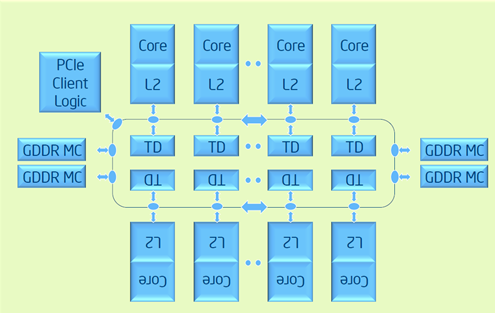
\includegraphics[width=0.6\textwidth]{figures/phi_arch.png}
    \caption{Intel Xeon Phi architecture\cite{opencl_phi}.}
    \label{PhiArch}
\end{figure}

\subsubsection{Mapping}
\begin{itemize}
    \item A \emph{work group} is the smallest task being scheduled on the threads\cite{opencl_phi}.
    \item At initialization time the Intel OpenCL driver creates 240 software threads and pins them to the hardware threads, then
        when you call \emph{clEnqueueNDRange()}, the intel driver schedules the \emph{work groups} of the current \emph{NDRange}
        into the 240 threads\cite{opencl_phi}.
    \item The OpenCL compiler implicitely vectorize the \emph{work group} routine based on dimension zero loop.
    \item The vector size is always 16, regardless of the data type used by the kernel. As OpenCL \emph{work items} are guaranteed
        to be independent, the OpenCL vectorizer needs no feasibility to apply vectorization. However the vectorized kernel is only
        used if the local size of dimension zero is greater or equal to 16(even for double precision floating point numbers?). 
        Otherwise, the OpenCL runtime runs the scalar kernel for each of the \emph{work items}. Also it is important to mention that
        if the \emph{work group} size at dimension zero is not divisible by 16, then the end of the \emph{work group} needs to be 
        executed by scalar version of the kernel\cite{opencl_phi}.
\end{itemize}


